% vim: tw=80

\chapter{The CMS Detector at the Large Hadron Collider}

\todo{beschleunigergeschichte cern}
LEP and Tevatron have provided remarkabable insights into the Standard Model and
precision tests of the Standard Model.

\section{The Large Hadron Collider}

The Large Hadron Collider (LHC) is the world's most powerful particle
accelerator and collider. The LHC is contained in the circular tunnel of the
preceding Large Electron Positron (LEP) collider which has a circumference of 27
km at a depth between 50 and 175 m. The tunnel crosses the border between
Switzerland and France at four points and two of the four main experiments are
located in Frace. 

Two adjacent beamlines that intersect at four interactions points contain the
particle beams travelling in opposite directions. More than 1000 dipole magnets,
generating a magnetic field of up to 8.3 T bend the proton beams on the circular track while
almost 400 quadrupole magnets keep the beams focused. 

The proton beams are brought to collision at four interaction points which house
the LHC experiments ALICE~\cite{ALICE}, ATLAS~\cite{ATLASa}, CMS and
LHCb~\cite{LHCb}. ALICE is designed to study the quark-gluon plasma produced by
colliding heavy ions, which resembles the initial state of the universe. LHCB is
precisely measuring the CP violation and the decay of B mesons. ATLAS and CMS,
general purpose detectors allowing a broad field of phycis studies, were built
to search and study the Higgs boson and physics models beyond the standard
model. Additionally precision measurements of standard model predictions and
parameters improve the current knowledge and the confidence of predictions of
the standard model.

Prior to the injection and acceleration of protons in the LHC, the particles
pass a series of consecutive acceleration steps succesively increasing their
energy. The linear particle accelerator (LINAC2) generates 50 MeV protons, that
are further accelerated in the Proton-Synchrotron (PS) to 26 GeV and
the Super-Proton-Synchrotron (SPS) up to an energy of \SI{450}{\giga
\electronvolt}. At last the proton beams are injected into the LHC ring and are
further accelerated up to peak design energy of 13 TeV. All these
pre-accelerators are not only used to feed the LHC, but also serve other physic
experiments as can be seen in Figure~\ref{fig:lhc_complex}.

\begin{figure}[htp]
    \centering
    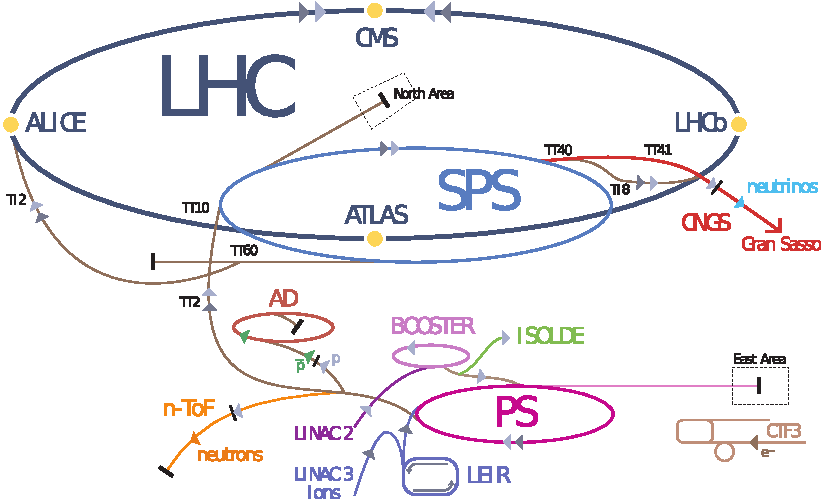
\includegraphics[width=0.8\textwidth]{figures/cms_detector/lhc_accelerator_chain.pdf}
    \caption[CERN accelerator complex]{Schematic view of the CERN
        accelerator complex. It shows the LHC ring  with the four beam crossing
        points as well as the various pre-accelerators~\cite{LHC:COMPLEX}.}
    \label{fig:lhc_complex}
\end{figure}

\subsection{The Compact Muon Solenoid Detector}

The Compact Muon Solenoid (CMS) detector is a general purpose detector at the
LHC located at Point 5, at the opposite side of the CERN campus at Meyrin. To
serve a vast range of physics studies, its design is driven by a cylyndrical
structure containing layers of different subdetectors each built
to measure a specific type of particles at high precision. A high-precision
inner tracking system is surrounded by an electromagnetic and hadronic
calorimeter which are encased by a superconducting solenoid magnet, and a high
precision muon detection system. The detector is 21.6 m long and 14.6 m in
diameter, weighing more than 12000 tons due to its compact design. The detector
was built as cylyndrical slices constructed at ground level and lowered into the
cavern. In case of upgrades or repairs, the slices can be pulled apart and easy
access to the inner components is gained. 

\begin{figure}[htp]
    \centering
    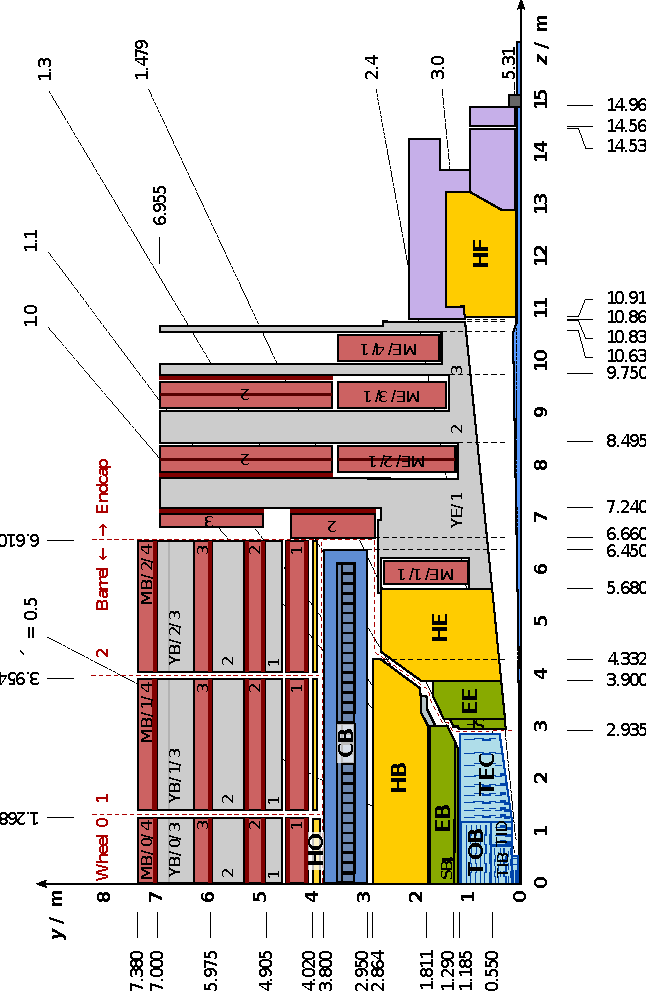
\includegraphics[width=0.8\textwidth]{figures/cms_detector/cms_longitudinal_section.pdf}
    \caption[Longitudinal section of the CMS detector]{asdf}
    \label{fig:cms:longitudinal_section}
\end{figure}

\todo{high requirements like 25 ns between collisions, high radiation level,
advanced detector materials.}

\subsection{Definition of the Coordinate System}

CMS uses a right-handed coordinate system centered at the nominal interaction point inside the
detector. The $x$-axis points radially inward towards the LHC ring centre, the
$y$-axis vertically upwards and the $z$-axis along the beam direction towards
the Jura mountains. Important quantities are the azimuthal angle $\phi$
measured from the $x$-axis in the $x$-$y$ plane and the polar angle $\theta$,
measured from the $z$-axis in the $z$-$y$ plane. Instead of the polar angle
$theta$, the pseudo-rapidity $\eta$ and the rapidity $y$ are commonly used to
split the phasespace, since the differential flux is approximately constant at
hadron-hadron colliders. The pseudo-rapidity is defined as

\begin{equation}
    \eta = - \ln \left( \tan \left( \frac{\theta}{2} \right) \right)
\end{equation}

Throughout this thesis the rapidity is favoured compared to the pseudo-rapidity
due to its invariance under longitudinal boosts in the $z$-direction. Rapidity
and pseudo-rapidity are equivalent in the case of massless particle. The
rapidity is defined as

\begin{equation}
    y = \frac{1}{2} \ln \left( \frac{E + p_z}{E - p_z} \right) 
\end{equation}

The momentum along the beamline is not well defined due to the momentum
distribution inside the proton. A direct connection to the hard process is given
by the transverse momentum \pt related to cartesian coordinates as

\begin{equation}
    \pt = \sqrt{p_x^2 + p_y^2}
\end{equation}

\subsection{Inner Tracking System}
\todo{measurement of charged particles.}

To yield a best possible spatial resolution, the particle tracks needs be
measured as close to the beam line as possible. The inner tracking system of CMS
is designed to measure the tracks of charged particles emerging from the
collision. Enclosing the interaction point with its diameter of 2.6 m and
extending 2.8 m in each direction of the beamline, the tracking system covers a
pseudo-rapidity range up to $|\eta| < 2.5$. 

The inner tracking system comprises two subsystems, the \textbf{silicon pixel
detector}, consisting of three layers and installed very close to the beam pipe,
and the silicon strip detector with ten layers in the barrel region. The pixel
detector contains 65 millon pixels arranged in three cylindrical layers at 4 cm,
7 cm and 11 cm to the beam pipe. The pixel detector is able to resolve the huge
number of particle tracks of around 10 million particles per square centimetre
and reconstruct their tracks. The high spatial resolution achieved by the pixel
detector additionally allows the identification and measurement of secondary
vertices used to identify long-lived particles.

Reduced particle flux further away from the beam pipe eases the identification
of tracks. Cost-efficient \textbf{silicon strip detectors} are employed reaching out to
an radius of 1.3 m. The strip detector consists of a total of 10 million
detecting strips read out by 80,000 chips. 

\begin{figure}[htp]
    \centering
    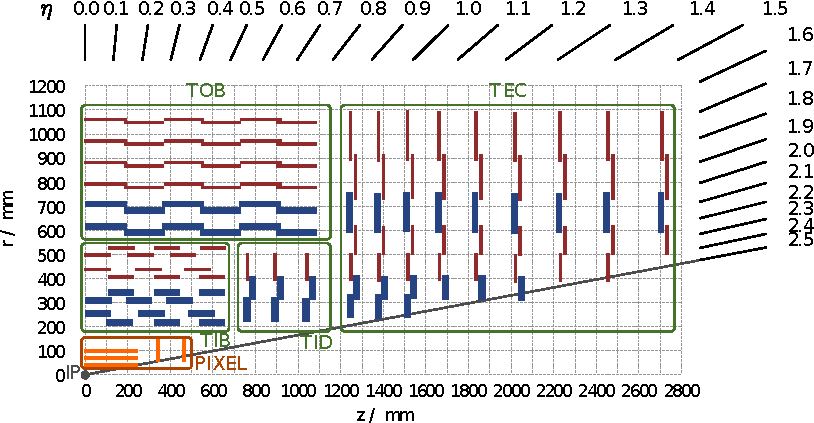
\includegraphics[width=0.65\textwidth]{figures/cms_detector/tracker.pdf}\hfill
    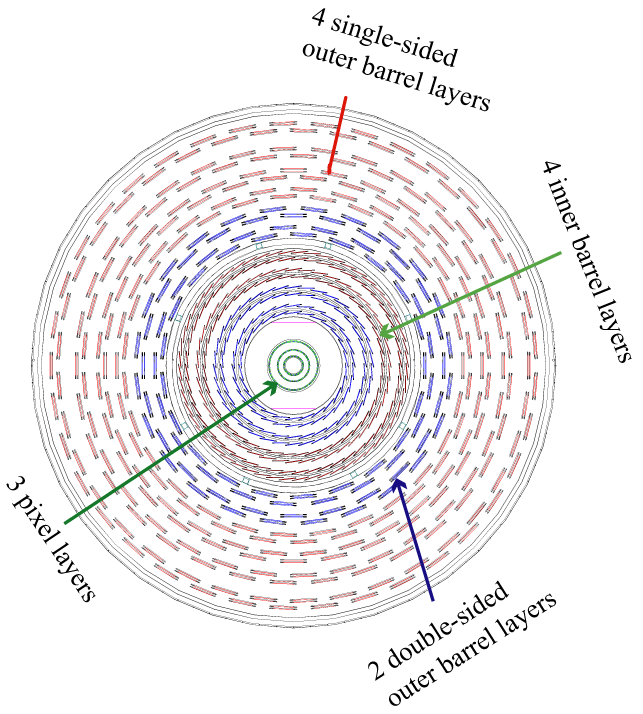
\includegraphics[width=0.3\textwidth]{figures/cms_detector/tracking_sytem_barrel_slice.png}
    \caption[Inner Tracking System]{The left figure shows one quadrant of the
        longitudinal section of the inner tracking system of CMS consisting of the
        silicon pixel detector and the silicon strip detector. The right figure shows a
        transverse section of the tracking system in the barrel region with overlapping
        arrangement of the strip modules. Figures from~\cite{phd:joramberger} and
        \cite{cmsweb:innertracker}.}
    \label{fig:cms:inner_tracking}
\end{figure}

\subsection{Electromagnetic Calorimeter}

Measuring the track of the traversing particles is not sufficient to derive to
measure the momentum. The energy needs to be measured by stopping the particles
in the detector and measuring the size of the deposited energy. The photon and
electron energy is measured in the electromagnetic calorimeter (ECAL). 

High-energetic photons, electrons or positrons which enter the dense material of the ECAL
detector, produce an electromagnetic shower via subsequent bremsstrahlung and
electron-pair production processes. Below a certain threshold, the particles
deposit their energy via compton scattering and the photo-electric effect in the
detector material resulting in an excitation of their atomic state. When they
return to the ground state, they emit photons, which can be measured using
avalanche photodiodes. The fraction of the deposited energy is to the number of
emitted photons.

The hermetic calorimeter is made of lead tungstate ($\mathrm{PbWO}_4$), a very
dense material with a radiation length of $X_0 = 0.89$ cm. Through the
additional oxygen, it is a highly transparent and scintillates light. These
material properties allow the calorimeter to be built very compact within the
solenoid magnet. Additionally, the small Moli`ere  radius of 2.19 cm leads to a
fine granularity. 

\begin{figure}[htp]
    \centering
    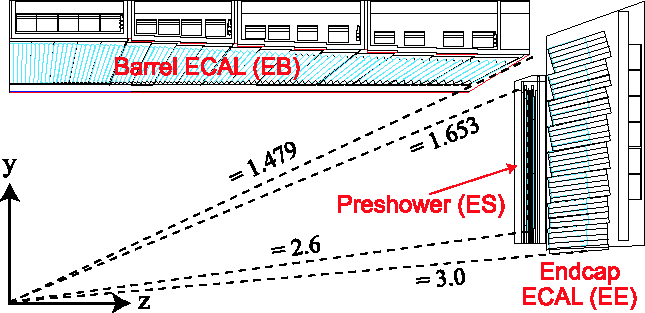
\includegraphics[width=0.8\textwidth]{figures/cms_detector/cms_ecal.pdf}\hfill
    \caption[Electromagnetic Calorimeter]{The electromagnetic calorimeter
    consists of two submodules covering the barrel regiond and the endcaps.
    Additionally a preshower detector is mounted in front of the
    endcaps~\cite{cms:ecal}.}
    \label{fig:cms:ecal}
\end{figure}

Figure~\ref{fig:cms:ecal} shows a schematic sketch of the ECAL in the $y$-$z$
plane. The ECAL consists of three subsystems covering the the pseudo-rapidity
range upt to 3.0. The \textbf{electromagnetic calorimeter barrel (EB)} covers up
to $\eta < 1.479$ using more than 60000 crystals forming a homogenous coverage
in pseudo-rapidity. Each crystal measures 2.2 cm x 2.2 cm x 23 cm corresponding
to a radiation length of 25.8 $X_0$. The \textbf{electromagnetic calorimeter
endcaps (EE)} extend the pseudo rapidity coverage from $1.479 < |\eta| < 3.0$.
The largest part of the ECAL endcap is additionally covered by the
\textbf{electromagnetic pre-shower detector (ES)}. It consists of two orthogonal
silicon strip sensors. The ES improves the discrimination between single
high-energetic photos and less interesting low-energy photon pairs as well as
the discrimination between neutral pions and photons.

The relative energy resolution of the ECAL can be parametrized using the NSC-formula

\begin{equation}
    \left( \frac{\sigma}{E} \right)^2 = \frac{N^2}{E^2} + \frac{S^2}{E} + C^2
\end{equation}

in which the first term describes the contribution by noise (N), the second
term the stochastic (S) component arising from the proportional relation between
the number of counted photons and the deposited energy and last a constant (C)
term.

\subsection{Hadronic Calorimeter}

The compact design of the CMS detector limits the size of the calorimeters. CMS
therefore built a sampling calorimeter inside the solenoid coil. The hadronic
calorimeter consists of brass as absorber material which is non-magnetic and
has a short interaction lenth of $\lambda_I = 16 \si{\centi\metre}$. It is
interleaved with plastic scintillators measuring the deposited energy. The CMS
hadronic calorimeter comprises three subsystems. The \textbf{Hadron Barrel
Calorimeter (HB)} covers the barrel region up to a pseudo-rapidity $|\eta| <
1.305$. The absorbing material in the barrel has a corresponding thickness of
$5.39 \lambda$ in the central region up to $10.3 \lambda$ at $|\eta| = 1.3$. The
HB is complemented by the \textbf{Hadron Outer Calorimeter (HO)} located on top
of the coil of the magnet. Using the coil as absorbing material it is able to
meaure the tails of hadron showers penetrating the HB and the coil.The
\textbf{Hadron Endcap Calorimeter (HE)} extends the pseudo-rapidity coverage up
to $|\eta| < 3.0$. A major challenge in the construction of the HE were the
usage of non-magnetic material to not disturb the magnetic field as well as the
close distance to the beampipe. Radiation damages decrease the detector response
and have to be corrected for continously. The \textbf{Hadron Forward (HF)}
calorimeter extends even closer to the beam pipe. With a coverage of $2.8 <
|\eta| < 5.2$ the calorimeter is adapted to the high radiation environment. The
HF is desinged using iron absorbers and quartz fibres as active material, which
measure the Cerenkov light emitted by the relativistic components of the
shower.

Hadrons entering the calorimeter produce a hadronice shower. High-energetic
hadrons mostly shower in inelatic interactions producing a large number of pions
and nucleans. Due to the large transverse momentum of these secondary particles,
hadronic shower spread further in the calorimeter than electromagnetic shower.
When the energy of the particles involved in the shower drops below a certain
theshold, the energy is deposited by ionisation and low-energy hadronic
activity. The active scintillation material is excitated eand emits blue-violet
light. The scintillators are connected to photodiodes using wavelength
shifters which read out the signals and pass it to the data aquisition system.

\subsection{Superconducting Solenoid}

A key component of the CMS detector is the superconductiong magnet which
produces a magnetic field of 4 T and is located inside the detector between the
calorimeters and the muon system. It measures a diameter of 6 m and a lenth of
12.5 m. When operated at design magnetic field strenth, the magnet contains an
energy of 2.6 GJ. The strong magnetic field is neccessary to bend the particle
tracks for a high momentum resolution in the tracking system. Operated at a
temperature of 4 K, the NbTi conductors become superconducting. The muon system
is installed within a 10,000 t iron yoke which return the magnetic field.

\subsection{Muon System}

Identifying and measuring muons with high precision is an unrivalled capacity of
the CMS detector. Unlike most other particles, muons are not stopped by the
calorimeters but leave the detector. Therefore, the muon system has been placed
around the other detector components to measure the bended tracks of the muons.

By combining the information of the inner tracking system and the muon
detectors, the path and the muon momentum can be measured precisely. The muon
system comprises three different types of detectors each suited for a specific
task. Drift tubes (DT) cover the barrel region up to $\eta < 1.2$, the endcaps
up to $\eta < 2.4$ are measured using cathode strip chambers (CSC) which also
work reliably in spatially varying magnetic field. The DT and CSC detectors
yield a precise spatial muon resolution. Both system are accompanied by
resistive plate chambers (RPC) which provide a fast response to the trigger
system.

\subsection{Trigger and Data Aquisition}

The LHC generates a huge number of collisions. At a beam crossing frequency of
25 ns, there are 40 million bunch crossings per second with an average of around
20 collisions per bunch crossing. With todays available hardware, the storage of
all collision data is not possible. Furthermore, most of the collisions are soft
and of low interest for physics analyses. Therefore a complex trigger system
consisting of a very fast hardware implemented component, the Level 1 trigger
(L1) and a software trigger, the High Level Trigger (HLT), analyses the incoming
data and decides if a collision event is of interest and should be stored
permanently or is omitted.

\begin{figure}[htp]
    \centering
    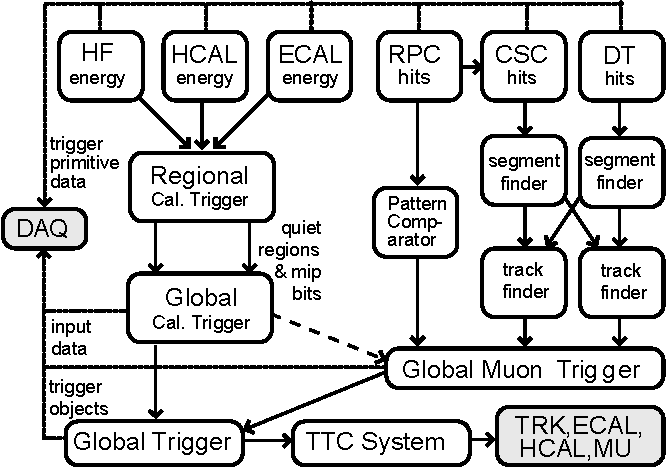
\includegraphics[width=0.8\textwidth]{figures/cms_detector/cms_l1_trigger.pdf}\hfill
    \caption[The L1 Trigger of CMS.]{asdf}
    \label{fig:cms:l1_trigger}
\end{figure}

When a collision occurs, the detector electronics is readout and directly
analyzed using custom hardware, the \textbf{L1 trigger}. Of special interest for
this thesis are the calorimeter triggers. Figure~\ref{fig:cms:l1_trigger} shows
the workflow of the L1. The Trigger Primitive Generators convert the frontend
electronics readout into transverse energy. The Regional Calorimeter Triggers
(RCT) identify electromagnetic shower in the ECAL and sum up the ECAL and HCAL
trigger tower. Additonally a patter recognition is performed to identify jets
and hadronic $\tau$ decays. These candidates are then passed to the Global
Calorimeter Trigger which sorts the incoming candidates from the all 18 regional
triggers and passes the top canadites to the Global Trigger (GT). If the global
trigger accepts the event it is further processed by the data aqusition system
and passed to the high level trigger.

the \textbf{High Level Trigger} is fully implemented in software running on a
dedicated computing farm at Point 5. The software is implemented in the CMS
reconstruction software and can therefore access all information from the whole
detector as well as aplly basic jet energy corrections. Jet Trigger for example
need to pass a \pt threshold on reconstructed calorimeter jets before complex
particle flow and jet reconstruction algorithm are performed to save processing
time.

The data aquisition system can apply prescales on each trigger to reduce the
rate at which a trigger fires. Especially for single jet triggers, which
trigger on the jet \pt, need to be prescaled in the low-\pt region to avoid huge
rates. Of course the trigger prescales have to be taken into account again when
the spectrum is reconstructed from the number of events.

\subsection{Data aquisition}

\section{Software and Computing Infrastructure}

% cmssw grid-control, root,

% physics software: herwig/pythia nlojt++/fastNLO:
